\subsection{Estado de resultados}
El estado de resultados es proyectado a 5 años, de forma que, se conoce a detalle los movimientos de dinero dentro de la empresa, teniendo en cuenta los costos para generar las utilidades netas del año fiscal.

En la tabla \ref{estado} se ilustra la utilidad bruta que se obtiene como resta entre ventas netas y el total de costo de ventas, también la utilidad operacional que es resultado de la utilidad bruta menos los gastos administrativos, por ultimo los gastos financieros y pre-operativos que generan la utilidad antes de impuestos resultado de la resta de impuestos de renta en el año gravable 2022.

\vspace{2mm}
\begin{minipage}{0.9\textwidth}
\centering
\captionof{table}[{Estado de resultados }]{ Estado de resultados }
\label{estado}
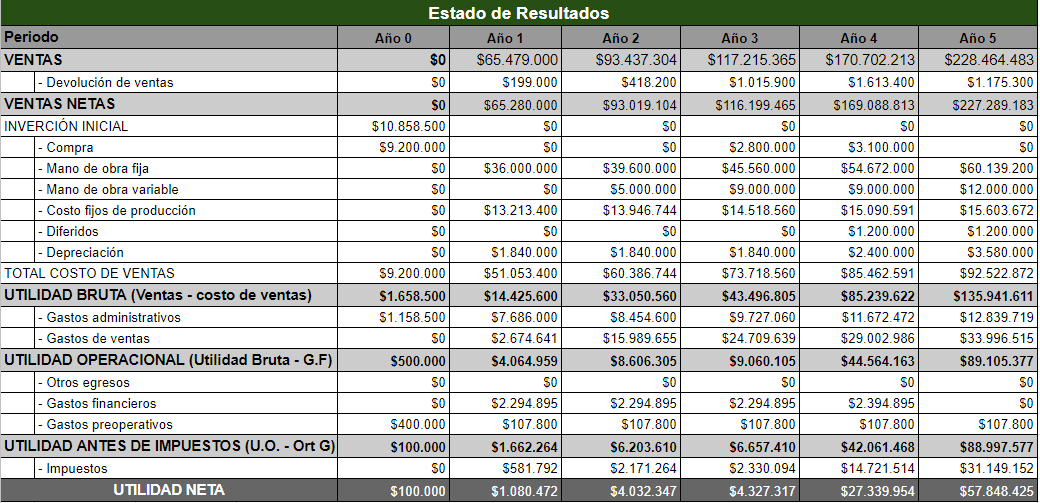
\includegraphics[width=1.1\textwidth]{Images/estadoResultados.png}
\fnote{Nota. \textup{Fuente : Autores}}
\end{minipage}
\newpage